\begin{figure}[htbp]
	\centering
	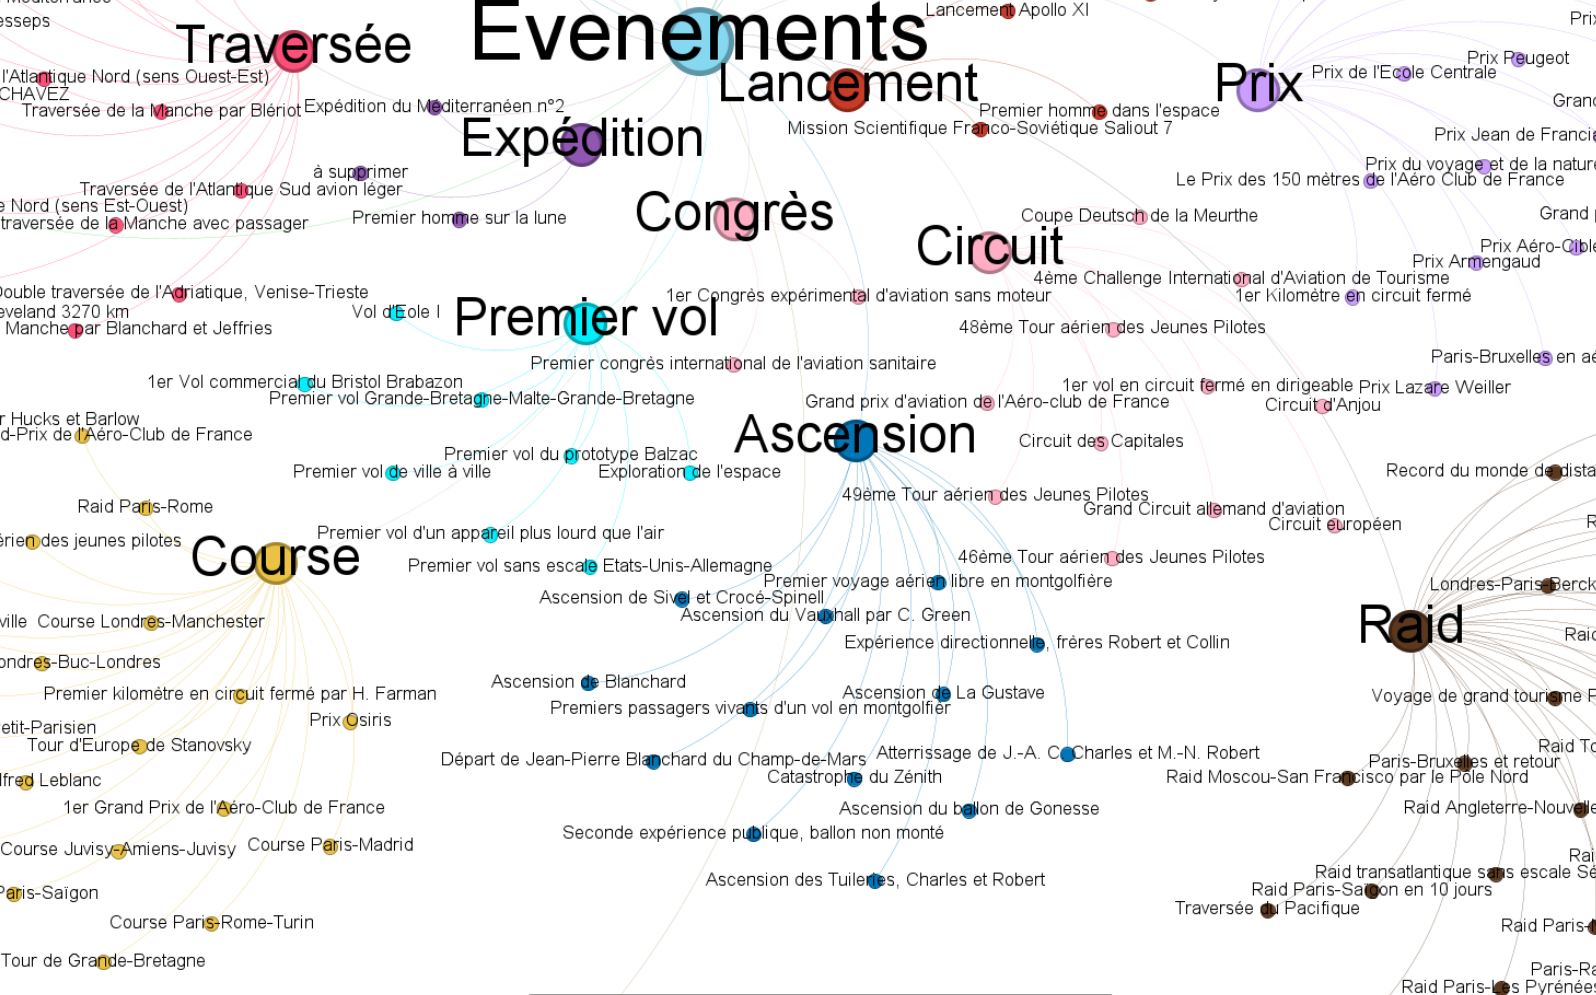
\includegraphics[width=\linewidth]{img/GRAPH_evenements}
	\caption[Modélisation en graphe du thésaurus des événements de l'e-médiathèque]{Modélisation en graphe du thésaurus des événements de l'e-médiathèque (réalisée avec \textit{Gephi})}
	\label{fig:graphevenements}
\end{figure}



\lettrine{L}{e} graphe ci-dessus offre une visualisation synthétique du thésaurus des événements indexés dans l'e-médiathèque du musée. Cette cartographie a permis de révéler plusieurs points d'analyse sur ce thésaurus, qui ont été regroupés ci-dessous à titre d'exemple et de manière non exhaustive :

\begin{itemize}
	
	\item \textbf{Juxtaposition des catégories principales} : les grands types d'événements (\enquote{Ascension}, \enquote{Course}, \enquote{Raid}, \enquote{Congrès}, \enquote{Lancement}, \enquote{Expédition}, \enquote{Premier vol}, \enquote{Traversée}, \enquote{Circuit} et \enquote{Prix}) coexistent tous sur un même niveau directement sous le terme de tête \enquote{Évènements}, sans appliquer la hiérarchie recommandée par les normes de gestion de thésaurus.
	
	\item \textbf{Hétérogénéité des noms} : la démarche choisie pour créer les entrées -- et donc la manière dont on doit \enquote{positionner} un événement en conséquence -- reste floue : on rencontre à la fois des catégories génériques, des intitulés d’événements particuliers, des formulations descriptives et des variantes typographiques. Cette absence de règles communes dans le nommage complique la recherche et fragilise la cohérence documentaire.
	
	Le graphe met en évidence de nombreuses incohérences de nommage : certaines relèvent d’un événement historique  (\enquote{Lancement}, \enquote{Ascension}), d’autres appartiennent au registre de l’action et sont difficiles à distinguer les unes des autres (\enquote{Course}, \enquote{Raid}, \enquote{Prix}) ; les termes spécifiques ne semblent pas obéir à des règles absolues en terme de normalisation (notamment pour ce qui est de la mention de noms propres).
	
	\item \textbf{Déséquilibre des branches} : certaines catégories (notamment \enquote{Course}, \enquote{Ascension}, \enquote{Raid}) concentrent un volume important de sous-événements, tandis que d'autres restent peu développées, ce qui peut révéler une structuration inégale du vocabulaire.
	
\end{itemize}


Cette modélisation permet d'établir un constat mitigé sur l'état de ce thésaurus : bien qu'il soit déjà construit, ne semble pas présenter un grand nombre d'anomalies (termes orphelins, doublons), de nombreuses améliorations en terme de normalisation, de hiérarchisation des termes et de clarification de leur signification et concept associés peuvent y être apportées.
Ce sont ces quelques points qui ont ainsi servi à guider le groupe de travail réalisé à ce sujet au \mae~et ont permis de proposer la hiérarchisation plus claire proposée dans le tableau de travail suivant.

\begin{figure}[htbp]
	\centering
	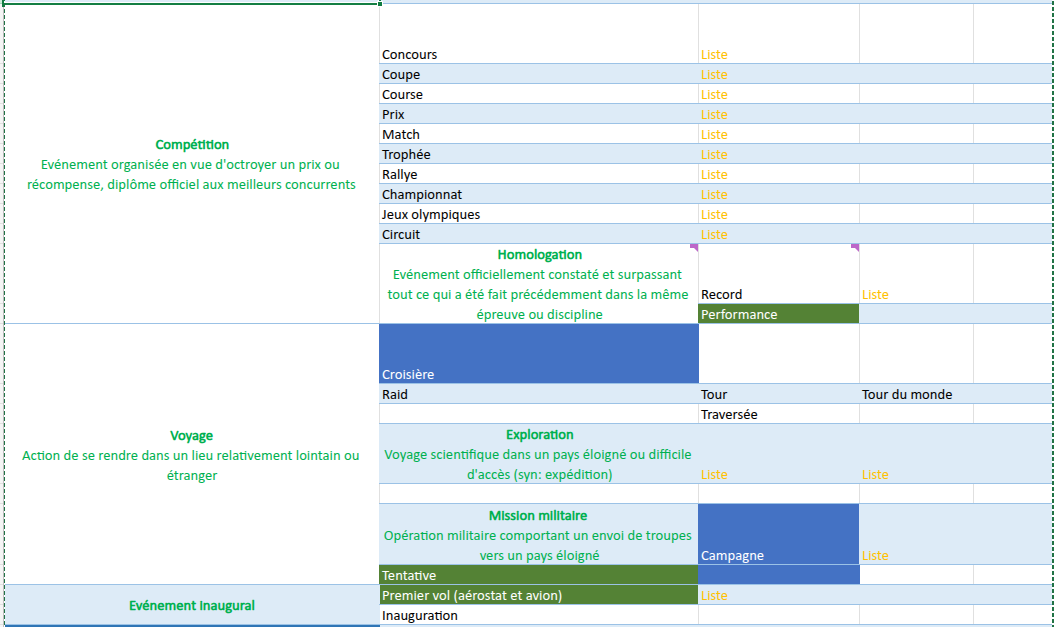
\includegraphics[width=\linewidth]{img/TABL_evenements}
	\caption[Proposition de rationalisation du thésaurus réalisée dans le cadre du groupe de travail sur les événements]{Proposition de rationalisation du thésaurus réalisée dans le cadre du groupe de travail sur les événements -- \textit{le tableau se lit de gauche à droite, les termes de tête étant dans la première colonne}.}
	\label{fig:tablevenements}
\end{figure}
